  \documentclass[a4paper,
fontsize=11pt,
%headings=small,
oneside,
numbers=noperiodatend,
parskip=half-,
bibliography=totoc,
final
]{scrartcl}

\usepackage{synttree}
\usepackage{graphicx}
\setkeys{Gin}{width=.8\textwidth} %default pics size

\graphicspath{{./plots/}}
\usepackage[ngerman]{babel}
\usepackage[T1]{fontenc}
%\usepackage{amsmath}
\usepackage[utf8x]{inputenc}
\usepackage [hyphens]{url}
\usepackage{booktabs} 
\usepackage[left=2.4cm,right=2.4cm,top=2.3cm,bottom=2cm,includeheadfoot]{geometry}
\usepackage{eurosym}
\usepackage{multirow}
\usepackage[ngerman]{varioref}
\setcapindent{1em}
\renewcommand{\labelitemi}{--}
\usepackage{paralist}
\usepackage{pdfpages}
\usepackage{lscape}
\usepackage{float}
\usepackage{acronym}
\usepackage{eurosym}
\usepackage[babel]{csquotes}
\usepackage{longtable,lscape}
\usepackage{mathpazo}
\usepackage[normalem]{ulem} %emphasize weiterhin kursiv
\usepackage[flushmargin,ragged]{footmisc} % left align footnote
\usepackage{ccicons} 
\usepackage{hyperxmp}

\usepackage{listings}

\urlstyle{same}  % don't use monospace font for urls

\usepackage[fleqn]{amsmath}

%adjust fontsize for part

\usepackage{sectsty}
\partfont{\large}

%Das BibTeX-Zeichen mit \BibTeX setzen:
\def\symbol#1{\char #1\relax}
\def\bsl{{\tt\symbol{'134}}}
\def\BibTeX{{\rm B\kern-.05em{\sc i\kern-.025em b}\kern-.08em
    T\kern-.1667em\lower.7ex\hbox{E}\kern-.125emX}}

\usepackage{fancyhdr}
\fancyhf{}
\pagestyle{fancyplain}
\fancyhead[R]{\thepage}

%meta

%meta

\fancyhead[L]{N. Jahn \& B. Kaden \\ %author
LIBREAS. Library Ideas, 31 (2017). % journal, issue, volume.
\href{http://nbn-resolving.de/}
{}} % urn
\fancyhead[R]{\thepage} %page number
\fancyfoot[L] {\ccLogo \ccAttribution\ \href{https://creativecommons.org/licenses/by/3.0/}{\color{black}Creative Commons BY 3.0}}  %licence
\fancyfoot[R] {ISSN: 1860-7950}

\title{\LARGE{Notiz zum Titelbild\\Über den Versuch, Stimmungen innerhalb von Kommentaren der Initiative Publikationsfreiheit zu bemessen}} %title %title
\author{Najko Jahn \& Ben Kaden} %author

\setcounter{page}{1}

\usepackage[colorlinks, linkcolor=black,citecolor=black, urlcolor=blue,
breaklinks= true,]{hyperref}

\hypersetup{%
      pdfcopyright={CC BY 4.0},
      pdflicenseurl={https://creativecommons.org/licenses/by/4.0/},
      baseurl={http://libreas.eu/}
     }

\date{}
\begin{document}

\maketitle
\thispagestyle{fancyplain} 

%abstracts

%body
Das Titelbild dokumentiert Empfindungen im Zuge der
Urheberrechtsnovellierung anhand der Kommentare der Unterstützer des
Appells \enquote{Publikationsfreiheit - für eine starke
Bildungsrepublik}\footnote{\url{https://www.publikationsfreiheit.de/}}.
Am 30. Juni hat der Bundestag Schrankenregelungen zur Nutzung
urheberrechtlich geschützter Werke in Bildung und Forschung reformiert,
die zum 1. März 2018 in Kraft treten werden. Einzelne Verleger wollten
mit dem Appell im Vorfeld der Abstimmung öffentlichkeitswirksam auf ihre
Anliegen hinweisen und forderten zugleich, das Reformvorhaben in die
nächste Legislaturperiode zu verschieben. Während der Appell seitens der
Frankfurter Allgemeinen Zeitung positiv aufgenommen wurde, warfen
Bibliothekare wie Eric Steinhauer der Kampagne eine Irreführung von
Wissenschaft, Politik und Öffentlichkeit vor. Zudem seien die
Unterzeichnerinnen und Unterzeichner des Appells nicht repräsentativ für
alle wissenschaftlich Beschäftigten an Hochschulen und
Forschungseinrichtungen in Deutschland.\footnote{\url{https://irights.info/artikel/publikationsfreiheitde-unterzeichner/28410}}

Was bleibt, sind bis dato 2.357 Kommentare der Unterzeichner des
Appells. Die Frage, die uns angesichts unseres Schwerpunkts
\enquote{Emotionen} beschäftigt hat, war, welche Stimmungen und
Empfindungen sich gegenüber der geplanten Urheberrechtsreform in den
Kommentaren ausdrücken und wie sie sich für ein Titelbild festhalten
lassen. Zu diesem Zwecke geeignet sind Sentimentanalysen. Die
Sentimentanalyse ist ein Verfahren des Text-Mining, das mit Methoden des
maschinellen Lernens, Aussagen als positiv oder negativ charakterisiert.
Voraussetzung ist ein Korpus, das positiv und negativ konnotierte Wörter
oder Wortgruppen enthält und entsprechend gewichtet. Zwar existieren
auch für die deutsche Sprache entsprechende Wortschätze.\footnote{z.B.
  SentiWS: \url{http://wortschatz.uni-leipzig.de/de/download}} Wir haben
uns jedoch aufgrund der einfachen Nachnutzung für die Text Analytics API
von Microsoft entschieden, die insbesondere auf die Unterstützung von
Kommunikationsprozessen in Unternehmen zielt und somit weniger für
wissenschaftliche Auswertungen geeignet ist.\footnote{\url{https://azure.microsoft.com/en-us/services/cognitive-services/text-analytics/}}
Die Umsetzung erfolgte mittels der statistischen Programmierumgebung R
als dynamischer Report in R Markdown\footnote{\url{https://github.com/libreas/ausgabe31/blob/master/notiz/master.Rmd}}
und folgt der Methodendarstellung im kürzlich erschienen Buch
\enquote{Text Mining with R - A Tidy Approach} von Julia Silge und David
Robinson.\footnote{\url{http://tidytextmining.com/}}

Nachfolgend beschreiben wir, wie wir die Daten gewonnen und die
Abbildung für das Titelbild visualisiert haben. Zunächst wurden die
Kommentare aus der Webseite der Initiative Publikationsfreiheit
extrahiert, Formatierungszeichen entfernt und ein Datensatz zum Abgleich
mit der Text Analytics API erstellt. Die Text Analytics API ist mittels
eines API-Keys zugriffsbeschränkt und ermöglicht je Aufruf die Analyse
von bis 1000 Textabschnitten.

Ergebnis ist eine Tabelle, die jedem Kommentar einen Wert zwischen 0
(negativ) und 1 (positiv) zuweist. Für die Abbildung wollten wir
allerdings 0 als neutralen Wert definieren und normalisierten den
Sentimentwert des Scores entsprechend einer neuen Skale, die von -0.5
bis +0.5 reicht.

Der so gewonnene Datensatz ist unter
\url{sentiment_publikationsfreiheit.csv} verfügbar. Die Sentimentwerte
wurden abschließend als Säulendiagramm visualisiert, das jeden Kommentar
mit seinem Sentimentwert abbildet:

\begin{figure}
\centering
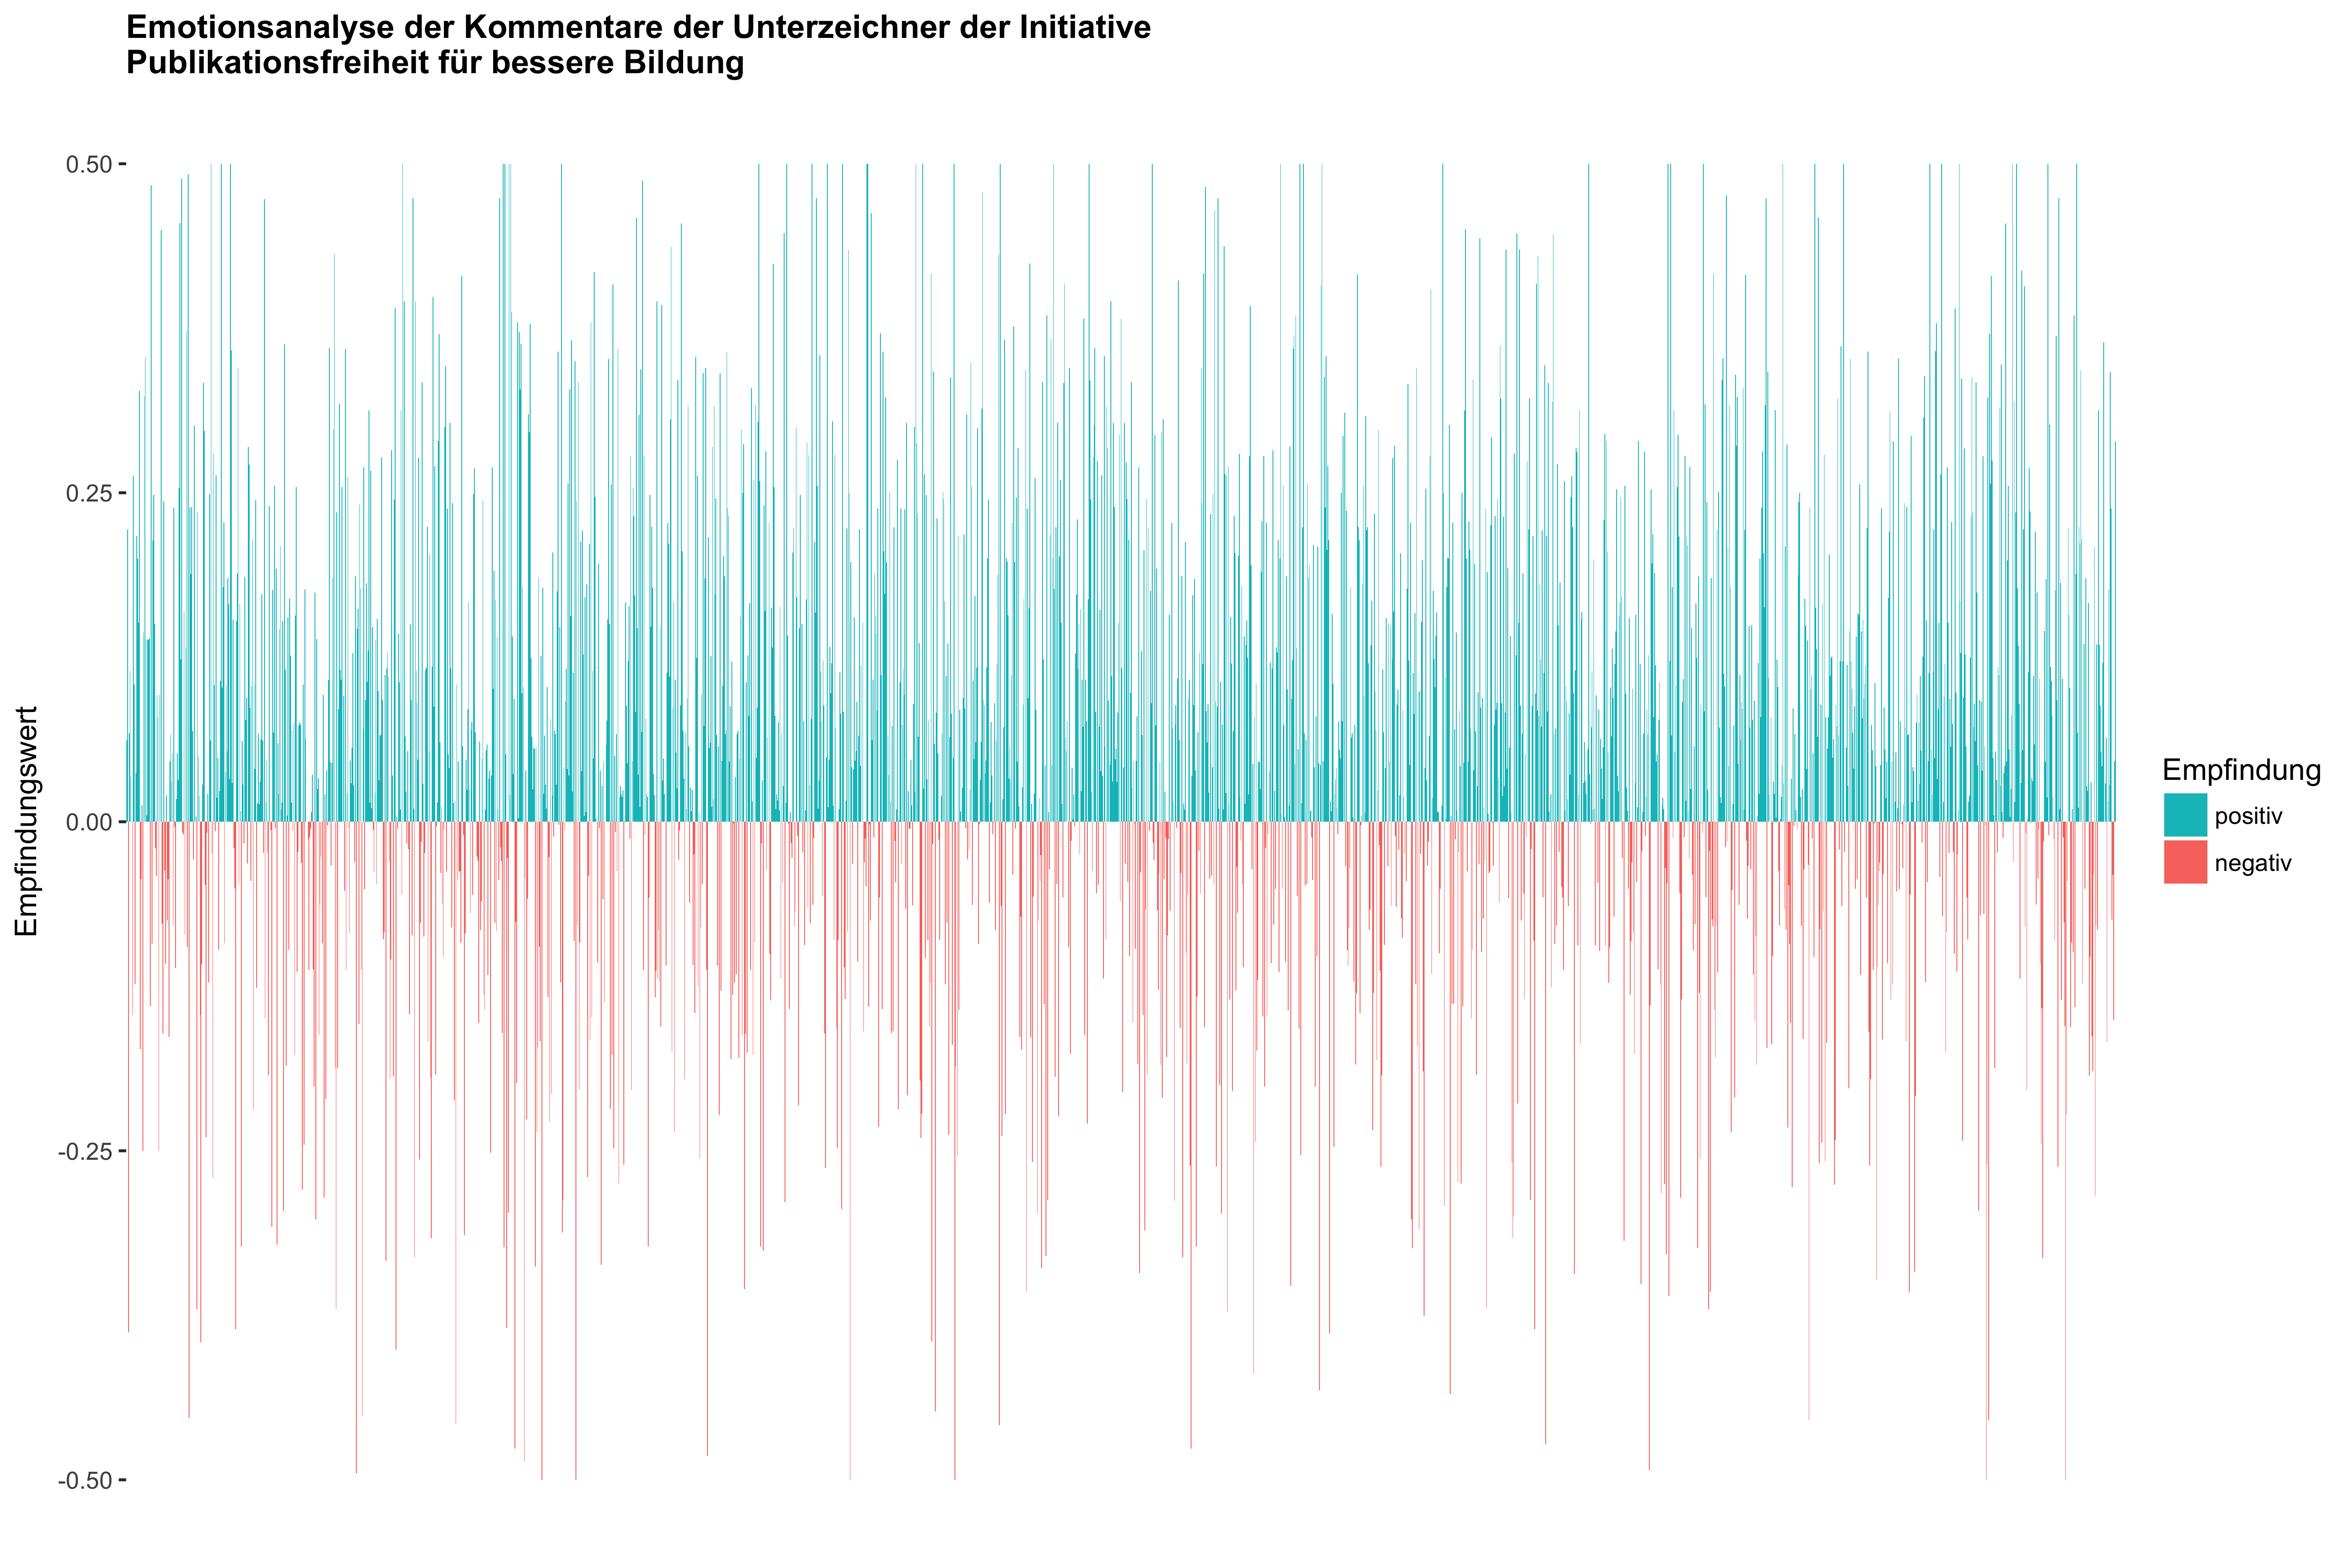
\includegraphics{img/sentiment_abbbildung.png}
\caption{Sentimentanalyse Appell Publikationsfreiheit}
\end{figure}

Es scheint, als wäre der Großteil der Kommentare neutral bis positiv
konnotiert. Extrem negative Aussagen blieben die Ausnahme. Das lässt
zunächst wenigstens vermuten, dass die rhetorische Gestaltung des
Aufrufs ihren Zweck sehr gut erfüllte. Der Appell an die Sicherung der
Grundwerte führte zu einer weitreichenden Bekräftigung derselben durch
die Unterzeichnenden in den Kommentaren. Beispiele sind: \enquote{Das
höchste Gut des Menschen ist Bildung und Freiheit, das muss bewahrt
werden.} Oder \enquote{{[}Ich unterstütze die Publikationsfreiheit,
weil{]} ich selbst frei schreiben möchte - und das Recht der freien
Meinungsäußerung als hohes Gut einer Demokratie ehre.} Oder:
\enquote{{[}Ich unterstütze die Publikationsfreiheit,{]} weil sie in
einer Demokratie, für Bildung und eine vielfältige Verlagslandschaft
unabdingbar ist.}

Bereits die Vorgabe \enquote{Ich unterstütze die Publikationsfreiheit,
weil\ldots{}} leitete assoziativ und fast zwangsläufig auf eine Bejahung
hin und zwar ungeachtet der Frage, ob die Auslegung des Konzeptes durch
die Initiatoren des Aufrufs auch dem entspricht, was die Kommentierenden
mit Publikationsfreiheit verbinden bzw. ob der Gesetzesentwurf
tatsächlich eine Bedrohung derselben darstellte. Die Bahn ist gelegt und
die Vorlage lädt ein, zu betonen, wie wichtig und gerechtfertigt die
Initiative ist.

Die als negativ ermittelten Aussagen sind oft leider wenig einleuchtend,
auch weil das Konzept Sentiment in diesem Rahmen zu unscharf
qualifiziert wird. Zugleich finden sich zahlreiche Aussagen, die in
ihrer Logik selbst eher fragwürdig sind. Ein Beispiel: \enquote{{[}Ich
unterstütze die Publikationsfreiheit, weil{]} ich damit befürchte, dass
der Weg zu TTIP, TiSa und Ceta geebnet werden soll/wird.} Aufmerksame
Lesende mögen hier schlussfolgern, dass der Kommentator nicht etwa
impliziert, dass die Publikationsfreiheit (=\enquote{damit}) TTIP
vorbereitet. Sondern vielmehr die Urheberrechtsreform. Aber es ist zu
bezweifeln, dass eine automatisierte Spracherkennung damit zurecht
kommt. Abgesehen davon, dass der Kommentar auch inhaltlich auf einer
sehr schiefen Bahn unterwegs ist.

Eine weitere notwendige Einschränkung ist also, dass das Verfahren
selbst zwar quantitativ sauber ist, die bekannten semantischen
Herausforderungen natürlichsprachlicher Kommunikation aber nur
eingeschränkt berücksichtigt. Der Blick ins Detail zeigt, wie sehr viele
Kommentare hinsichtlich der Konnotationsermittlung tatsächlich eine
intellektuelle Interpretation benötigten. Bei nicht wenigen der
Kommentare ermöglicht auch diese keine eindeutige Zuordnung. Aussagen
wie: \enquote{\ldots{}ich nicht möchte, dass die Leistung von AutorInnen
und Verlagen entwertet wird} werden vom verwendeten sprachanalytischen
Cloud-Dienst als stärker negativ eingeschätzt. Die Aussage
\enquote{\ldots{}ich in den Plänen der Bundesregierung zum Urheberrecht
eine massive Bedrohung der Wissenschaftsfreiheit sehe} wird dagegen eher
überraschend als stärker positiv bewertet. \enquote{Ich unterstütze die
Publikationsfreiheit, weil vor allem Bildung wichtig ist} tendiert wider
Erwarten ins Negative. Zwei Dinge lassen sich daraus schlussfolgern:
Einerseits ist die Stimmung nicht immer so eindeutig, dass sie sich in
wenigen Schritten algorithmisch sauber und nachvollziehbar sortieren
lässt. Und daher, zweitens, eignen sich Verfahren wie das Beschriebene
mit ihrem aktuellen Stand vor allem dazu, Auffälligkeiten zu
identifizieren, denen man über eine qualitative Folgeanalyse nachspüren
kann. Wir laden unsere Leserinnen und Leser herzlich dazu ein und
erklären uns gern bereit, entsprechende Arbeiten in kommenden Ausgaben
von LIBREAS oder auch im LIBREAS. Weblog nachzureichen.

%autor
\begin{center}\rule{0.5\linewidth}{\linethickness}\end{center}

\textbf{Najko Jahn} ist Datenanalyst an der Nidersächsischen Staats- und
Universitätsbibliothek Göttinen und Redaktionsmitglied der LIBREAS.

\textbf{Ben Kaden} ist Bibliothekswissenschaftler an der
Universitätsbibliothek der Humboldt-Universität zu Berlin und
Mitherausgeber von LIBREAS

\end{document}